\documentclass[11pt, a4paper]{article}

\usepackage[utf8]{inputenc}
\usepackage[T1]{fontenc}
\usepackage[catalan, provide=*]{babel}
\usepackage[protrusion=true,expansion=false]{microtype}
\usepackage{geometry}
\geometry{top=2.5cm, bottom=2.5cm, left=2.8cm, right=2.8cm}
\usepackage{amsmath, amssymb, amsthm}
\usepackage{mathtools}
\usepackage{enumitem}
\usepackage{tikz}
\usetikzlibrary{arrows.meta, calc}
\usepackage{fancyhdr}
\pagestyle{fancy}
\fancyhf{}
\fancyhead[L]{\small Desaparcament autom\`atic en paral$\cdot$lel}
\fancyhead[R]{\small Taller de Modelitzaci\'o --- UAB}
\fancyfoot[C]{\thepage}
\renewcommand{\headrulewidth}{0.4pt}
\usepackage[colorlinks=true,linkcolor=black,citecolor=black,urlcolor=black]{hyperref}

\theoremstyle{plain}
\newtheorem{theorem}{Teorema}[section]
\newtheorem{lemma}[theorem]{Lema}
\newtheorem{proposition}[theorem]{Proposici\'o}
\theoremstyle{definition}
\newtheorem{definition}[theorem]{Definici\'o}
\newtheorem{remark}[theorem]{Observaci\'o}
\newtheorem{hypothesis}[theorem]{Hip\`otesi}

\newcommand{\Ro}{R_o}

\title{%
  \large Universitat Aut\`onoma de Barcelona\\
  Grau en Matem\`atiques --- Taller de Modelitzaci\'o\\[1em]
  \LARGE\bfseries Desaparcament Autom\`atic en Paral$\cdot$lel\\[0.3em]
  \large Un algorisme geom\`etric per a un nombre arbitrari de passos
}
\author{David Elias \and \'Alvaro Noya \and Xavier Parellada \and Guillem Sala}
\date{Juny de 2026}

\begin{document}
\maketitle\thispagestyle{empty}

\begin{abstract}
Aquest treball presenta un algorisme geom\`etric per desaparcar un vehicle
de dimensions $L\times W$ d'una pla\c{c}a d'aparcament en paral$\cdot$lel de
dimensions $A\times B$, tenint en compte el principi d'Ackermann i l'angle
m\`axim de gir $\delta_0$ de les rodes davanteres. Es defineix formalment el
model cinem\`atic, s'estableix la posici\'o inicial i es demostra que, sota
la hip\`otesi $B>L$, l'algorisme termina en un nombre finit de passos.
Es caracteritza tamb\'e la condici\'o geom\`etrica que permet la sortida
despr\'es d'un \'unic Pas~1.
\end{abstract}

\tableofcontents\newpage

%──────────────────────────────────────────────────────────────────────────────
\section{Introducci\'o i objectius}

L'aparcament en paral$\cdot$lel \'es una de les maniobres m\'es exigents per
a un conductor. La pregunta que ens plantegem \'es la inversa: donat un vehicle
ja aparcat, com pot sortir de la pla\c{c}a de manera autom\`atica, i en quants
passos?

Per la reversibilitat dels moviments r\'igids al pla, dissenyar un algorisme
de desaparcament \'es equivalent a resoldre el problema de l'aparcament
autom\`atic~\cite{AA2023}. Treballem doncs amb el problema de desaparcament,
que \'es geom\`etricament m\'es c\`omoda d'analitzar des de la posici\'o
inicial fixada.

Donats $L$, $W$, $\delta_0$, $A$, $B$, volem un algorisme que:
\begin{enumerate}[noitemsep]
  \item decideixi si el vehicle pot desaparcar, i
  \item en cas afirmatiu, l'hi faci indicant el nombre de passos necessaris.
\end{enumerate}

El treball s'organitza com seg\"ueix. La Secci\'o~\ref{sec:model} estableix
el model cinem\`atic. La Secci\'o~\ref{sec:posicio} defineix la posici\'o
inicial. La Secci\'o~\ref{sec:algorisme} presenta l'algorisme. La
Secci\'o~\ref{sec:1pas} tracta la condici\'o de sortida en un pas. La
Secci\'o~\ref{sec:terminacio} demostra la terminaci\'o en el cas general.
La Secci\'o~\ref{sec:conclusions} recull les conclusions.

%──────────────────────────────────────────────────────────────────────────────
\section{Model cinem\`atic}\label{sec:model}

\subsection{Vehicle i pla\c{c}a}

Modelitzem el vehicle com un rectangle de llargada $L$ i amplada $W$.
Les quatre rodes s\'on: $r_{pd}$ (posterior dreta), $r_{pe}$ (posterior
esquerra), $r_{dd}$ (davantera dreta), $r_{de}$ (davantera esquerra).

La pla\c{c}a d'aparcament \'es un rectangle de llargada $B$ (en la direcci\'o
del moviment inicial del vehicle) i amplada $A$ (perpendicular). Els obstacles
s\'on:
\begin{itemize}[noitemsep]
  \item \textbf{Paret del fons} ($y=0$): darrere del vehicle.
  \item \textbf{Cotxe de davant} ($y=B$, per $\Ro+\frac{W}{2}-A \leq x
        \leq \Ro+\frac{W}{2}$): limita el moviment endavant dins la pla\c{c}a.
  \item \textbf{Vorera de la dreta} ($x > \Ro+\frac{W}{2}$): a la dreta
        de les rodes dretes.
  \item \textbf{Obertura cap a la carretera}: la banda esquerra de la
        pla\c{c}a, recta $\ell: x = \Ro+\frac{W}{2}-A$, per $y\geq 0$.
\end{itemize}

\begin{definition}[Pas]\label{def:pas}
Un \emph{pas} \'es una parella $(\delta,d)\in(0,\delta_0]\times\mathbb{R}^*$
on $\delta$ \'es l'angle de gir de la roda interior davantera i $d$ la
dist\`ancia d'arc recorreguda pel punt mig de l'eix posterior. Si $d>0$ el
vehicle avan\c{c}a; si $d<0$ recul$\cdot$la. Una \emph{maniobra} \'es una
successi\'o finita de passos.
\end{definition}

\begin{remark}
Treballarem sempre amb $\delta=\delta_0$ (gir m\`axim), ja que maximitza
el despl\c{c}ament lateral per unitat de dist\`ancia recorreguda.
\end{remark}

\subsection{Principi d'Ackermann}

\begin{proposition}[Ackermann]\label{prop:ackermann}
Quan el vehicle gira, els eixos de les quatre rodes es tallen en un \'unic
centre instant\`ani de rotaci\'o $O$, situat sobre la prolongaci\'o de l'eix
posterior. Si $\delta_{int}$ i $\delta_{out}$ s\'on els angles de la roda
interior i exterior davanteres:
\[
  \cot\delta_{out} - \cot\delta_{int} = \frac{W}{L}.
\]
\end{proposition}

\begin{proof}
Sigui $X$ la dist\`ancia horitzontal de $O$ a la roda interior. Per
definici\'o, $\tan\delta_{int}=L/X$ i $\tan\delta_{out}=L/(X+W)$. Llavors:
\[
  \cot\delta_{out}-\cot\delta_{int}
  =\frac{X+W}{L}-\frac{X}{L}=\frac{W}{L}.\qedhere
\]
\end{proof}

Fixat $\delta_0$, el radi de gir del punt mig de l'eix posterior \'es:
\[
  \Ro = L\cot\delta_0.
\]
Els radis de les rodes davanteres quan el vehicle gira a l'esquerra
(roda interior $=$ dreta) s\'on:
\[
  R_{dd} = \sqrt{\!\Bigl(\Ro+\tfrac{W}{2}\Bigr)^{\!2}+L^2}, \qquad
  R_{de} = \sqrt{\!\Bigl(\Ro-\tfrac{W}{2}\Bigr)^{\!2}+L^2}.
\]
Com que $\Ro+W/2>\Ro-W/2\geq 0$, tenim $R_{dd}>R_{de}$: la roda $r_{dd}$
\'es la primera a tocar el cotxe de davant durant el gir cap a l'esquerra.

\begin{figure}[h]
\centering
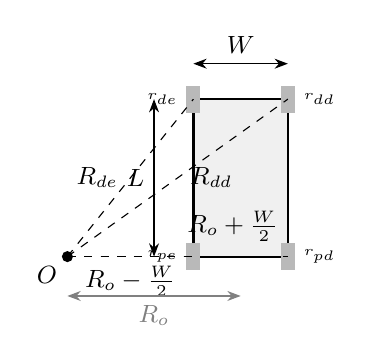
\begin{tikzpicture}[scale=1.0,>=Stealth,thick]
  % Ro=2.2, W=1.2, L=2.0 -> xl=Ro-W/2=1.6, xr=Ro+W/2=2.8
  % car body
  \fill[gray!12](1.6,0) rectangle (2.8,2.0);
  \draw(1.6,0) rectangle (2.8,2.0);
  % wheels
  \foreach \wx/\wy in {1.6/0, 2.8/0, 1.6/2.0, 2.8/2.0}{
    \fill[gray!55](\wx-0.09,\wy-0.17) rectangle (\wx+0.09,\wy+0.17);}
  % origin
  \fill(0,0) circle (2pt);
  \node[below left,font=\small] at (0,0){$O$};
  % radii
  \draw[dashed,thin](0,0)--(1.6,0)
    node[midway,below,font=\small]{$\Ro-\tfrac{W}{2}$};
  \draw[dashed,thin](0,0)--(2.8,0)
    node[near end,above=2pt,font=\small]{$\Ro+\tfrac{W}{2}$};
  \draw[dashed,thin](0,0)--(1.6,2.0)
    node[midway,left=1pt,font=\small]{$R_{de}$};
  \draw[dashed,thin](0,0)--(2.8,2.0)
    node[midway,right=1pt,font=\small]{$R_{dd}$};
  % dims
  \draw[<->,thin](1.1,0)--(1.1,2.0)
    node[midway,left,font=\small]{$L$};
  \draw[<->,thin](1.6,2.45)--(2.8,2.45)
    node[midway,above,font=\small]{$W$};
  \draw[<->,thin,gray](0,-0.5)--(2.2,-0.5)
    node[midway,below,gray,font=\small]{$\Ro$};
  % roda labels
  \node[right=2pt,font=\tiny] at (2.8,0){$r_{pd}$};
  \node[left=2pt,font=\tiny]  at (1.6,0){$r_{pe}$};
  \node[right=2pt,font=\tiny] at (2.8,2.0){$r_{dd}$};
  \node[left=2pt,font=\tiny]  at (1.6,2.0){$r_{de}$};
\end{tikzpicture}
\caption{Geometria d'Ackermann. El centre de rotaci\'o $O$ \'es sobre la
prolongaci\'o de l'eix posterior, a dist\`ancia $\Ro=L\cot\delta_0$ del punt
mig. Com que $R_{dd}>R_{de}$, la roda $r_{dd}$ \'es la primera a tocar el
cotxe de davant.}
\label{fig:ackermann}
\end{figure}

%──────────────────────────────────────────────────────────────────────────────
\section{Posici\'o inicial i sistema de coordenades}\label{sec:posicio}

\begin{definition}[Posici\'o inicial]\label{def:posinicial}
Col$\cdot$loquem el sistema de coordenades de manera que el centre de rotaci\'o
$O$, quan el vehicle gira al m\`axim cap a l'esquerra des de la posici\'o
inicial, sigui l'origen $O=(0,0)$. Situem el vehicle paral$\cdot$lel a la
pla\c{c}a, amb les rodes posteriors sobre $y=0$ i les rodes dretes ajustades
a la dreta (a dist\`ancia de seguretat de la vorera). Les coordenades de les
quatre rodes s\'on:
\begin{align*}
  r_{pd}^{(0)}&=\bigl(\Ro+\tfrac{W}{2},\ 0\bigr), &
  r_{pe}^{(0)}&=\bigl(\Ro-\tfrac{W}{2},\ 0\bigr),\\
  r_{dd}^{(0)}&=\bigl(\Ro+\tfrac{W}{2},\ L\bigr), &
  r_{de}^{(0)}&=\bigl(\Ro-\tfrac{W}{2},\ L\bigr).
\end{align*}
\end{definition}

La pla\c{c}a t\'e amplada $A$ (par\`ametre independent) i la banda esquerra
de la pla\c{c}a, que \'es l'obertura cap a la carretera, \'es la recta:
\[
  \ell:\; x = \Ro+\frac{W}{2}-A.
\]
Notem que, com que les rodes dretes estan a $x=\Ro+W/2$ i la pla\c{c}a
t\'e amplada $A$, la paret esquerra de la pla\c{c}a se situa efectivament
a $x = (\Ro+W/2) - A$, consistent amb la definici\'o de $\ell$.

\begin{remark}
En general $A\neq \Ro+W/2$, de manera que $\ell$ no coincideix amb l'eix
$y$. El centre de rotaci\'o $O=(0,0)$ \'es un punt de la recta que cont\'e
l'eix posterior del vehicle; en general no pertany a $\ell$.
\end{remark}

\begin{figure}[h]
\centering
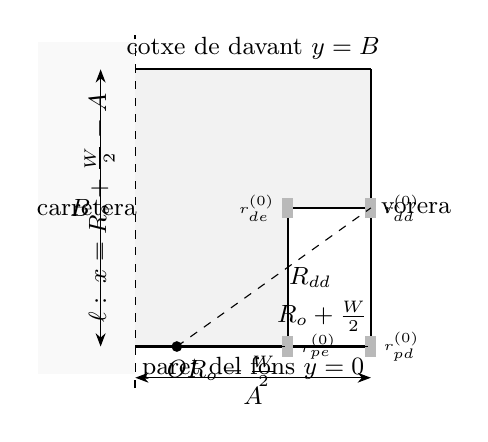
\begin{tikzpicture}[scale=0.88,>=Stealth,thick]
  % Ro=2.2, W=1.2, L=2.0, A=3.4, B=4.0
  % xl = Ro-W/2 = 1.6, xr = Ro+W/2 = 2.8
  % ell: x = xr - A = 2.8 - 3.4 = -0.6
  \def\ellx{-0.6}
  \def\Bv{4.0}
  \def\xr{2.8}
  \def\xl{1.6}
  \def\Lv{2.0}
  \def\Av{3.4}

  % parking spot: x in [ellx, xr], y in [0, B]
  \fill[gray!10](\ellx,0) rectangle (\xr,\Bv);
  \draw(\ellx,0)--(\xr,0);           % fons
  \draw(\xr,0)--(\xr,\Bv);           % paret dreta
  \draw(\ellx,\Bv)--(\xr,\Bv);       % cotxe de davant
  \draw[dashed](\ellx,-0.6)--(\ellx,{\Bv+0.5}); % ell
  % road (left of ell)
  \fill[gray!5](-2.0,-0.4) rectangle (\ellx,{\Bv+0.4});

  % car initial position
  \fill[white](\xl,0) rectangle (\xr,\Lv);
  \draw(\xl,0) rectangle (\xr,\Lv);
  % wheels
  \foreach \wx/\wy in {1.6/0, 2.8/0, 1.6/2.0, 2.8/2.0}{
    \fill[gray!55](\wx-0.08,\wy-0.15) rectangle (\wx+0.08,\wy+0.15);}

  % origin O
  \fill(0,0) circle (2.2pt);
  \node[below,font=\small] at (0,-0.05){$O$};

  % ell line label
  \node[rotate=90,above,font=\small] at ({\ellx-0.15},{\Bv/2})
    {$\ell:\;x=\Ro+\tfrac{W}{2}-A$};

  % radius to r_pe (= Ro-W/2 = 1.6)
  \draw[dashed,thin](0,0)--(\xl,0)
    node[midway,below,font=\small]{$\Ro-\tfrac{W}{2}$};
  % radius to r_pd (= Ro+W/2 = 2.8)
  \draw[dashed,thin](0,0)--(\xr,0)
    node[near end,above=2pt,font=\small]{$\Ro+\tfrac{W}{2}$};
  % radius to r_dd
  \draw[dashed,thin](0,0)--(\xr,\Lv)
    node[midway,right=2pt,font=\small]{$R_{dd}$};

  % roda labels
  \node[right=1pt,font=\tiny] at (\xr,0){$r_{pd}^{(0)}$};
  \node[right=1pt,font=\tiny] at (\xl,0){$r_{pe}^{(0)}$};
  \node[right=1pt,font=\tiny] at (\xr,\Lv){$r_{dd}^{(0)}$};
  \node[left=1pt,font=\tiny]  at (\xl,\Lv){$r_{de}^{(0)}$};

  % dims
  \draw[<->,thin]({\ellx-0.5},0)--({\ellx-0.5},\Bv)
    node[midway,left,font=\small]{$B$};
  \draw[<->,thin](\ellx,-0.45)--(\xr,-0.45)
    node[midway,below,font=\small]{$A$};

  % wall labels
  \node[above,font=\small] at ({(\ellx+\xr)/2},\Bv)
    {cotxe de davant $y=B$};
  \node[below,font=\small] at ({(\ellx+\xr)/2},0)
    {paret del fons $y=0$};
  \node[right,font=\small]  at (\xr,\Bv/2){vorera};
  \node[font=\small] at (-1.3,\Bv/2){carretera};
\end{tikzpicture}
\caption{Sistema de coordenades i posici\'o inicial. $O=(0,0)$ \'es el
centre de rotaci\'o, situat sobre l'eix posterior del vehicle. La l\'inia
de sortida $\ell: x=\Ro+W/2-A$ \'es la banda esquerra de la pla\c{c}a.
En general $\ell$ no passa per $O$.}
\label{fig:posinicial}
\end{figure}

%──────────────────────────────────────────────────────────────────────────────
\section{L'algorisme de desaparcament}\label{sec:algorisme}

\subsection{Hip\`otesis}

\begin{hypothesis}\label{hyp:B}
$B > L$: la pla\c{c}a \'es m\'es llarga que el vehicle. Si $B\leq L$, el
vehicle no pot girar sense tocar simult\`aniament la paret del fons i el
cotxe de davant.
\end{hypothesis}

\begin{hypothesis}\label{hyp:A}
$A > W$: la pla\c{c}a \'es m\'es ampla que el vehicle, de manera que les
rodes dretes no toquen la paret esquerra.
\end{hypothesis}

\begin{hypothesis}\label{hyp:carril}
Un cop el vehicle ha sortit de la pla\c{c}a, el pas final (quedar
paral$\cdot$lel al carrer girant a la dreta) no produeix cap col$\cdot$lisi\'o
amb les parets de la pla\c{c}a ni amb la paret del fons.
\end{hypothesis}

\begin{remark}
La Hip\`otesi~\ref{hyp:carril} \'es una simplificaci\'o est\`andard
\cite{Vorobieva2012}. La seva verificaci\'o geom\`etrica queda com a treball
futur.
\end{remark}

\subsection{Definici\'o de desaparcar}

\begin{definition}[Sortida i desaparcament]\label{def:sortida}
Direm que el vehicle \emph{pot sortir} en l'instant $t$ si la roda $r_{dd}$
ha creuat la l\'inia $\ell$, \'es a dir,
\[
  x_{dd}(t) < \Ro + \frac{W}{2} - A.
\]
Direm que el vehicle \emph{ha desaparcat} quan, a m\'es, ha completat el
pas final: ha girat al m\`axim cap a la dreta i avan\c{c}at fins a quedar
paral$\cdot$lel al carrer.
\end{definition}

\begin{remark}
Fem servir $r_{dd}$ com a criteri de sortida perqu\`e $R_{dd}>R_{de}$:
\'es la \'ultima roda davantera a creuar $\ell$, i per tant \'es la condici\'o
m\'es restrictiva. Un cop $r_{dd}$ ha creuat $\ell$, la
Hip\`otesi~\ref{hyp:carril} garanteix que el pas final \'es possible.
\end{remark}

\subsection{Descripci\'o de l'algorisme}

\begin{enumerate}[label=\textbf{Pas \arabic*.},leftmargin=*,noitemsep]
\item \textbf{(Endavant-esquerra.)} Girar al m\`axim cap a l'esquerra
  ($\delta_{int}=\delta_0$) i avan\c{c}ar fins a una de dues condicions:
  \begin{enumerate}[label=(\alph*),noitemsep]
    \item $r_{dd}$ creua $\ell$: el vehicle pot sortir.
          S'executa el Pas~F i l'algorisme termina.
    \item $r_{dd}$ toca $y=B$: s'executa el Pas~2.
  \end{enumerate}
\item \textbf{(Enrere-dreta.)} Girar al m\`axim cap a la dreta i recular
  fins que $r_{pd}$ toca $y=0$. Tornar al Pas~1.
\end{enumerate}
\begin{enumerate}[label=\textbf{Pas F.},leftmargin=*]
\item[]\textbf{(Pas final.)} Girar al m\`axim cap a la dreta i avan\c{c}ar
  fins a quedar paral$\cdot$lel al carrer.
\end{enumerate}

\begin{figure}[h]
\centering
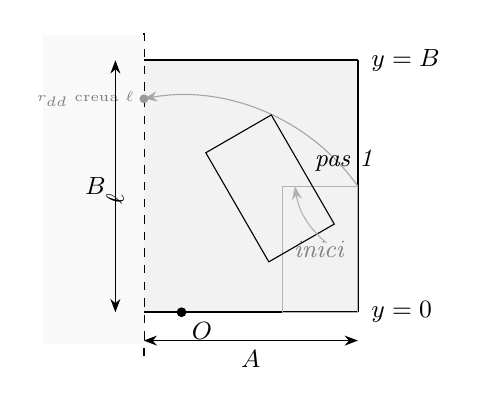
\begin{tikzpicture}[scale=0.80,>=Stealth,thick]
  % Ro=2.2, W=1.2, L=2.0, A=3.4, B=4.0
  % xl=1.6, xr=2.8, ellx=-0.6
  % Rdd = sqrt(2.8^2 + 2^2) = sqrt(7.84+4) = sqrt(11.84) ~ 3.44
  % phi0 = arctan(2/2.8) ~ 35.5 deg
  % r_dd crosses ell (x=-0.6) when Rdd*cos(phi0+theta) = -0.6
  % cos(phi0+theta*) = -0.6/3.44 ~ -0.174 => phi0+theta* ~ 100 deg => theta* ~ 64.5 deg
  \def\ellx{-0.6}
  \def\Bv{4.0}
  \def\xr{2.8}
  \def\xl{1.6}
  \def\Lv{2.0}
  \def\Rddv{3.44}
  \def\phiz{35.5}  % phi0 in degrees

  % spot
  \fill[gray!10](\ellx,0) rectangle (\xr,\Bv);
  \draw(\ellx,0)--(\xr,0);
  \draw(\xr,0)--(\xr,\Bv);
  \draw(\ellx,\Bv)--(\xr,\Bv);
  \draw[dashed](\ellx,-0.7)--(\ellx,{\Bv+0.5});
  \fill[gray!5](-2.2,-0.5) rectangle (\ellx,{\Bv+0.4});

  % initial car (gray)
  \draw[gray!60,thin](\xl,0) rectangle (\xr,\Lv);
  \node[gray,font=\small] at ({(\xl+\xr)/2},{\Lv/2}){\textit{inici}};

  % Arc of r_dd: from angle phi0=35.5 to angle ~100 deg (when x=-0.6)
  \draw[thin,->,gray!70]
    (\xr,\Lv) arc[start angle=\phiz, end angle=100, radius=\Rddv];
  % mark where r_dd crosses ell
  % at angle 100 deg: x=3.44*cos(100)~-0.60, y=3.44*sin(100)~3.39
  \fill[gray!80]({3.44*cos(100)},{3.44*sin(100)}) circle (2pt);
  \node[left,font=\tiny,gray] at ({3.44*cos(100)},{3.44*sin(100)})
    {$r_{dd}$ creua $\ell$};

  % Intermediate car: rotated ~30 deg around O
  \begin{scope}[rotate=30]
    \draw[thin](\xl,0) rectangle (\xr,\Lv);
  \end{scope}
  \node[font=\small] at (2.6,2.4){\textit{pas 1}};

  % Arrow
  \draw[->,thin,gray!60]
    ({(\xl+\xr)/2+0.1},{\Lv*0.55}) to[bend left=20] (1.8,2.0);

  % Origin
  \fill(0,0) circle (2.2pt);
  \node[below right,font=\small] at (0,0){$O$};

  % dims
  \draw[<->,thin]({\ellx-0.45},0)--({\ellx-0.45},\Bv)
    node[midway,left,font=\small]{$B$};
  \draw[<->,thin](\ellx,-0.45)--(\xr,-0.45)
    node[midway,below,font=\small]{$A$};
  \node[right,font=\small] at ({\xr+0.05},\Bv){$y=B$};
  \node[right,font=\small] at ({\xr+0.05},0){$y=0$};
  \node[rotate=90,font=\small,above] at ({\ellx-0.15},{\Bv*0.45})
    {$\ell$};
\end{tikzpicture}
\caption{Pas~1: el vehicle gira al m\`axim cap a l'esquerra (centre $O$).
La roda $r_{dd}$ descriu un arc de radi $R_{dd}$ fins a creuar $\ell$.
La condici\'o de sortida en un sol Pas~1 \'es que $r_{dd}$ arribi a $\ell$
sense haver tocat $y=B$.}
\label{fig:pas1}
\end{figure}

%──────────────────────────────────────────────────────────────────────────────
\section{Condici\'o de sortida en un sol Pas~1}\label{sec:1pas}

\subsection{C\`alcul de l'angle de sortida}

Durant el Pas~1, el vehicle gira al voltant de $O=(0,0)$ en sentit antihorari.
La posici\'o de $r_{dd}$ despr\'es d'una rotaci\'o d'angle $\theta\geq 0$ \'es:
\[
  r_{dd}(\theta) = R_{dd}
  \begin{pmatrix}\cos(\varphi_0+\theta)\\\sin(\varphi_0+\theta)\end{pmatrix},
  \qquad
  \varphi_0 = \arctan\!\frac{L}{\Ro+\tfrac{W}{2}}.
\]
La roda $r_{dd}$ creua $\ell: x=\Ro+W/2-A$ quan:
\[
  R_{dd}\cos(\varphi_0+\theta^*) = \Ro+\frac{W}{2}-A,
\]
\'es a dir:
\[
  \theta^* = \arccos\!\left(\frac{\Ro+\tfrac{W}{2}-A}{R_{dd}}\right) - \varphi_0.
\]
En aquell moment, la coordenada $y$ de $r_{dd}$ \'es:
\[
  y_{dd}(\theta^*) = R_{dd}\sin(\varphi_0+\theta^*)
  = R_{dd}\sqrt{1-\left(\frac{\Ro+\tfrac{W}{2}-A}{R_{dd}}\right)^{\!2}}
  = \sqrt{R_{dd}^2 - \Bigl(\Ro+\tfrac{W}{2}-A\Bigr)^{\!2}}.
\]
Substituint $R_{dd}^2 = (\Ro+W/2)^2+L^2$:
\[
  y_{dd}(\theta^*) = \sqrt{(\Ro+\tfrac{W}{2})^2+L^2-(\Ro+\tfrac{W}{2}-A)^2}
  = \sqrt{2A\!\left(\Ro+\tfrac{W}{2}\right)-A^2+L^2}.
\]
Expandint $(\Ro+W/2)^2 - (\Ro+W/2-A)^2 = 2A(\Ro+W/2) - A^2$:
\[
  \boxed{y_{dd}(\theta^*) = \sqrt{L^2 + 2A\!\left(\Ro+\tfrac{W}{2}\right) - A^2}.}
\]

\subsection{Condici\'o de no-col$\cdot$lisi\'o}

La coordenada $y$ de $r_{dd}$ al llarg del Pas~1 \'es
$y_{dd}(\theta)=R_{dd}\sin(\varphi_0+\theta)$, que \'es estrictament creixent
per $\theta\in[0,\,\pi/2-\varphi_0+\arcsin(A/R_{dd}-\ldots)]$.
Concretament, $y_{dd}$ creix fins que $r_{dd}$ arriba al punt m\'es alt del seu
arc, i despr\'es decreix. Per\`o $\theta^*$ \'es l'angle en qu\`e $r_{dd}$
creua $\ell$, i la coordenada $y$ en aquell punt \'es $y_{dd}(\theta^*)$
calculada m\'es amunt. Cal verificar que $y_{dd}$ \'es creixent fins a
$\theta^*$, \'es a dir, que $r_{dd}$ no ha passat pel seu punt m\'es alt
($\varphi_0+\theta=\pi/2$) abans de creuar $\ell$:
\[
  \varphi_0+\theta^* \leq \frac{\pi}{2}
  \iff \Ro+\frac{W}{2}-A \geq 0
  \iff A \leq \Ro+\frac{W}{2}.
\]
Si $A>\Ro+W/2$, llavors $r_{dd}$ passa pel seu punt m\'es alt \emph{abans}
de creuar $\ell$, i per tant $y_{dd}(\theta^*)$ no \'es el m\`axim de $y_{dd}$
en $[0,\theta^*]$: el m\`axim \'es $R_{dd}$, assolit a $\theta=\pi/2-\varphi_0$.
En aquest cas, la condici\'o de no-col$\cdot$lisi\'o \'es $R_{dd}<B$, \'es a
dir $(\Ro+W/2)^2+L^2<B^2$.

Resumint els dos casos:

\begin{theorem}[Condici\'o de sortida en un Pas~1]\label{thm:1pas}
Sota les Hip\`otesis~\ref{hyp:B}--\ref{hyp:carril}, el vehicle pot sortir
despr\'es d'un \'unic Pas~1 si i nom\'es si la m\`axima alc\`ada assolida per
$r_{dd}$ durant el Pas~1 \'es estrictament inferior a $B$. Concretament:
\begin{enumerate}[noitemsep,label=(\roman*)]
  \item Si $A\leq\Ro+W/2$: el m\`axim de $y_{dd}$ \'es assolit en creuar
        $\ell$, i la condici\'o \'es:
        \[
          \sqrt{L^2+2A\!\left(\Ro+\tfrac{W}{2}\right)-A^2} < B.
        \]
  \item Si $A>\Ro+W/2$: el m\`axim de $y_{dd}$ \'es $R_{dd}$, assolit
        abans de creuar $\ell$, i la condici\'o \'es:
        \[
          \sqrt{\left(\Ro+\tfrac{W}{2}\right)^{\!2}+L^2} < B.
        \]
\end{enumerate}
\end{theorem}

\begin{proof}
Per a cada $\theta\in[0,\theta^*]$, la coordenada $y_{dd}(\theta)=R_{dd}
\sin(\varphi_0+\theta)$. Aquesta funci\'o \'es creixent per
$\varphi_0+\theta<\pi/2$ i decreixent per $\varphi_0+\theta>\pi/2$.

\emph{Cas (i):} $A\leq\Ro+W/2$ implica $\Ro+W/2-A\geq 0$, i per tant
$\cos(\varphi_0+\theta^*)=(\Ro+W/2-A)/R_{dd}\geq 0$, \'es a dir
$\varphi_0+\theta^*\leq\pi/2$. La funci\'o $y_{dd}$ \'es doncs creixent en
tot $[0,\theta^*]$ i el m\`axim \'es $y_{dd}(\theta^*)=
\sqrt{L^2+2A(\Ro+W/2)-A^2}$.

\emph{Cas (ii):} $A>\Ro+W/2$ implica $\varphi_0+\theta^*>\pi/2$, de manera
que $y_{dd}$ primer creix fins a $R_{dd}$ (a $\theta=\pi/2-\varphi_0$) i
despr\'es decreix fins a $y_{dd}(\theta^*)$. El m\`axim \'es $R_{dd}=
\sqrt{(\Ro+W/2)^2+L^2}$.

En tots dos casos, la condici\'o de no-col$\cdot$lisi\'o amb $y=B$ \'es que
el m\`axim sigui $<B$.
\end{proof}

\begin{remark}
En el cas~(i) i usant $\Ro+W/2=A$ (vehicle ajustat al m\`axim), la condici\'o
es simplifica a $\sqrt{L^2+A^2}<B$, \'es a dir $L^2+A^2<B^2$. Usant la
relaci\'o $\Ro=A-W/2$ i expandint $2A(\Ro+W/2)-A^2 = 2A\cdot A - A^2 = A^2$,
que recupera $\sqrt{A^2+L^2}<B$.

Per a $A<\Ro+W/2$ (vehicle no ajustat al m\`axim), el terme
$2A(\Ro+W/2)-A^2$ \'es m\'es gran que $A^2$ (ja que $\Ro+W/2>A$), de manera
que la condici\'o \'es m\'es restrictiva: calen places m\'es llargues si el
vehicle no est\`a ben ajustat.
\end{remark}

%──────────────────────────────────────────────────────────────────────────────
\section{Terminaci\'o en el cas general}\label{sec:terminacio}

Quan el vehicle no pot sortir en un sol Pas~1, cal iterar el cicle
Pas~1/Pas~2. Demostrem que l'algorisme termina.

\begin{definition}\label{def:psi}
Definim $\psi_n\in[0,\pi/2)$ com l'angle que forma l'eix longitudinal del
vehicle amb la direcci\'o $y$ al principi del cicle $n$-\`esim ($\psi_0=0$).
\end{definition}

\begin{lemma}[Monot\'onia estricta]\label{lem:mono}
La successi\'o $(\psi_n)_{n\geq 0}$ \'es estrictament creixent.
\end{lemma}

\begin{proof}
Al Pas~1 del cicle $n$, el vehicle gira un angle $\Delta_n^+>0$ en sentit
antihorari fins que $r_{dd}$ toca $y=B$; per tant $\psi$ passa a
$\psi_n+\Delta_n^+$.

Al Pas~2, el vehicle recul$\cdot$la girant cap a la dreta un angle
$\Delta_n^->0$ fins que $r_{pd}$ toca $y=0$. Al final del Pas~1, la roda
$r_{pd}$ est\`a a una alc\`ada estrictament positiva $y_{pd}^+>0$ (s'ha
alc\c{c}at durant el gir cap a l'esquerra). Per tornar-la a $y=0$ reculant,
cal girar menys del que s'ha girat al Pas~1 (es recorre un arc menor per
baixar des de $y_{pd}^+$ fins a $0$, que per arribar des de $0$ fins a
$y_{pd}^+$). Per tant $\Delta_n^-<\Delta_n^+$ i:
\[
  \psi_{n+1} = \psi_n+\Delta_n^+-\Delta_n^- > \psi_n.
\]

\textit{Nota}: l'argument que $\Delta_n^-<\Delta_n^+$ usa la simetria
geom\`etrica del gir circular i el fet que $y_{pd}^+>0$, per\`o no hem
calculat expl\'icitament el nou centre de rotaci\'o al Pas~2 per verificar-ho
anal\'iticament. Aix\`o queda com a treball futur.
\end{proof}

\begin{theorem}[Terminaci\'o]\label{thm:terminacio}
Sota les Hip\`otesis~\ref{hyp:B}--\ref{hyp:carril} i amb $B>L$, l'algorisme
termina en un nombre finit de cicles.
\end{theorem}

\begin{proof}
Per el Lema~\ref{lem:mono}, $(\psi_n)$ \'es estrictament creixent i acotada
per $\pi/2$, de manera que convergeix a algun $\psi^*\leq\pi/2$.

Quan l'orientaci\'o del vehicle al principi del Pas~1 \'es $\psi_n$, la
condici\'o de sortida del Teorema~\ref{thm:1pas} dep\`en de la posici\'o
de $r_{dd}$ en les coordenades girades. A mesura que $\psi_n$ creix, el
vehicle est\`a m\'es girat cap a la sortida: la dist\`ancia que ha de recorrer
$r_{dd}$ per creuar $\ell$ disminueix, i la m\`axima alc\`ada de $r_{dd}$
durant el Pas~1 tamb\'e disminueix. Quan $\psi_n\to\pi/2$, el vehicle
est\`a gaireb\'e horitzontal i qualsevol petit avan\c{c} porta $r_{dd}$ a
creuar $\ell$, amb $y_{dd}\to 0 < B$. Per tant existeix $N$ tal que per a tot
$n\geq N$ es compleix la condici\'o de sortida i l'algorisme termina.

\textit{Nota}: l'argument que la m\`axima alc\`ada de $r_{dd}$ tendeix a $0$
quan $\psi_n\to\pi/2$ \'es geom\`etricament plausible per\`o no hem demostrat
que $\psi_n\to\pi/2$ (podria convergir a algun $\psi^*<\pi/2$ sense que la
condici\'o de sortida s'assoleixi mai). Tancar aquest buit requereix mostrar
que $\psi^*=\pi/2$ o que la condici\'o de sortida es compleix per a tot
$\psi_n>\psi_{\min}$ per algun $\psi_{\min}<\pi/2$. Aix\`o queda com a
treball futur.
\end{proof}

%──────────────────────────────────────────────────────────────────────────────
\section{Resum dels resultats}\label{sec:resum}

\begin{theorem}[Resultat principal]\label{thm:principal}
Sota les Hip\`otesis~\ref{hyp:B}--\ref{hyp:carril}:
\begin{enumerate}[noitemsep,label=(\roman*)]
  \item El vehicle pot sortir en un \'unic Pas~1 si i nom\'es si la m\`axima
        alc\`ada de $r_{dd}$ durant el Pas~1 \'es $<B$ (vegeu
        Teorema~\ref{thm:1pas}).
  \item En cas contrari, l'algorisme itera el cicle Pas~1/Pas~2, i termina
        en un nombre finit de cicles (sota les notes del
        Teorema~\ref{thm:terminacio}).
  \item La condici\'o necessari\`a per a qualsevol nombre de passos \'es
        $B>L$.
\end{enumerate}
\end{theorem}

%──────────────────────────────────────────────────────────────────────────────
\section{Conclusions}\label{sec:conclusions}

Hem presentat un algorisme geom\`etric per desaparcar un vehicle d'una
pla\c{c}a en paral$\cdot$lel, basat en el principi d'Ackermann. Els resultats
principals s\'on:
\begin{enumerate}[noitemsep]
\item \textbf{Model formal.} Definici\'o rigorosa del model cinem\`atic,
  posici\'o inicial i l\'inia de sortida $\ell: x=\Ro+W/2-A$.
\item \textbf{Condici\'o de sortida en un Pas~1.}
  Caracteritzaci\'o exacta en funci\'o de si $A\leq$ o $>\Ro+W/2$.
\item \textbf{Progr\'es monot\`on.} La successi\'o $(\psi_n)$ \'es
  estrictament creixent en cada cicle.
\item \textbf{Buits oberts.} La terminaci\'o en temps finit i el
  c\`alcul del nombre exacte de passos queden com a treballs futurs.
\end{enumerate}

Com a continuaci\'o: (a)~tancar el buit de la demostraci\'o de terminaci\'o;
(b)~derivar una f\'ormula del nombre de passos; (c)~verificar la
Hip\`otesi~\ref{hyp:carril}; (d)~relaxar la hip\`otesi d'ajust m\`axim a
la dreta.

\section*{Declaraci\'o d'\'us d'Intel$\cdot$lig\`encia Artificial}
En l'elaboraci\'o d'aquest treball s'ha fet \'us del model de llengua Claude
(Anthropic) com a assistent de redacci\'o, verificaci\'o de c\`alculs i
generaci\'o del codi \LaTeX. Tots els resultats han estat revisats pels autors.

\begin{thebibliography}{9}
\bibitem{AA2023}
J.\,J.~Rodr\'iguez Potosí, M.~Garc\'ia Mu\~noz, E.~Gonz\'alez Yu,
J.~Mar\'in M\'endez,
\textit{Aparcament Autom\`atic},
Taller de Modelitzaci\'o, UAB, 2023.
\bibitem{Vorobieva2012}
H.~Vorobieva, S.~Glaser, N.~Minoiu-Enache, S.~Mammar,
\textit{Geometric Path Planning for Automatic Parallel Parking in Tiny Spots},
13th IFAC Symp.\ Control in Transportation Systems, Sofia, 2012, pp.\,36--42.
\end{thebibliography}

\end{document}
